\section{Trapping the particle}\label{sec:4:trapping}
The presence of a shield introduces potential challenges to the stability of the particle trap. 
Levitated particles are typically trapped and cooled in ultra-high vacuum using magnetic, optical or electrical radiofrequency Paul traps \cite{GonzalezBallestero_2021}.
These traps differ in the trapping mechanism, but if the particle is cooled close to the ground state, all trapping potentials can be considered \q{harmonic} with trapping frequency $\omega_\mathrm{trap} = 2\pi \times f$.
The strength of the trapping potential $V \propto f^2$ varies across trap types, with frequencies typically ranging from $1\si{Hz}-1\si{kHz}$ for magnetic traps \cite{Slezak_2018} up to $10\si{kHz}-300\si{kHz}$ for optical traps \cite{GonzalezBallestero_2021}. 

If the particle is positioned close to the shield, the Casimir interaction may destabilize the trap or pull the particle onto the shield. The total potential $V_\mathrm{tot}=V_\mathrm{trap} + V_\mathrm{Casimir}$ is shown in \cref{fig:4:trap-eigenstates} for stable and unstable configurations.
\begin{figure}[!htbp]
  \centering
  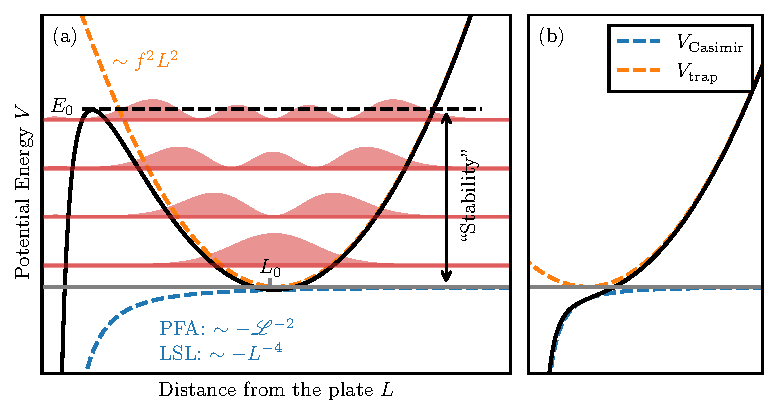
\includegraphics[width=\textwidth]{./../figures/others/trapping-potential-eigenstates.pdf}
  \caption{Visualization of the potential as an overlay of the harmonic trapping potential $V_\mathrm{trap} = m (2\pi f)^2 L^2 / 2$ and the Casimir potential $V_\mathrm{Casimir}$. $f$ is the trapping frequency and $L_0$ the position of the trap. In red, eigenstates of the potential are visualized offset by the eigen-energies.
  \textbf{(a)} Almost harmonic bounded potential which can hold the particle, if its energy is less than $E_0$.
  \textbf{(b)} Potential with no bounded states. Here, trapping is not possible.}
  \label{fig:4:trap-eigenstates}
\end{figure}
The attractive Casimir force $-\nabla V_\mathrm{Casimir}$ displaces the equilibrium trap position closer to the shield by a distance $\Delta x$ given by
\begin{equation}
  \Delta x = \frac{\abs{-\nabla V_\mathrm{Casimir}}}{m (2\pi f)^2} = \frac{2 \hbar c \pi^3}{720} \left(\frac{\varepsilon_r - 1}{\varepsilon_r + 1}\right) \varphi(\varepsilon_r) \frac{R}{\mathscr{L}^3} \frac{1}{m (2\pi f)^2} .
\end{equation}
For $f=1\si{kHz}$ and $L = 2R = 20\si{\mu m}$, this shift is negligibly small, as it is in the order of $\Delta x \approx 10^{-13}\si{m}$.

To determine the stability of a trapped particle with mass $M \propto R^3$ in a trap with frequency $f$ placed at a distance $L_0 > R$ in front of the shield, the number of bound energy-eigenstates in the potential $V_\mathrm{tot}$ is considered.
From \cref{fig:4:trap-eigenstates} it becomes clear, that as long as the particles thermal energy is well below $E_0$, the trap is stable and the particle is bound.
Here, $E_0$ is defined as the local maximum of the potential 
\begin{equation}
  E_0 = \max_{\substack{L\in(R,L_0) \\ \partial_L V(L) = 0}} \left( V_\mathrm{trap} + V_\mathrm{Casimir} \right) .
\end{equation}
If no such local maximum exists, i.e.
\begin{equation}
  \pdv{L} \left( V_\mathrm{trap} + V_\mathrm{Casimir} \right) \neq 0
\end{equation}
for all $L \in (R, L_0)$, the trap is unstable.
Regions of instability are shown in white in the stability diagram \cref{fig:4:trap-stability}.
In the general case, the stability can be measured by computing the number of bound eigenstates $n(E \leq E_0)$ and comparing them with the number of thermally excited states $\bar{n}$.
At a temperature $T$ on average 
\begin{equation}
  \bar{n} = \frac{1}{e^{\beta \hbar \omega} - 1}
\end{equation}
states are occupied, where $\beta = 1/k_B T$ and $\omega = 2\pi f$. This is true, as long as the potential is assumed to be harmonic, which is, as seen shortly, a good approximation.
To find the number of possible bound energy-eigenstates in the potential, the \emph{WKB-approximation} is used.
In this approximation, the energy $E$ of the $n$-th eigenstate of a smooth and appropriately slow varying potential $V(x)$ can be calculated using \cite[p. 163]{Schleich_2001}
\begin{equation}
  \int\limits_{x_1}^{x_2} \dd x \, \sqrt{2m(E-V(x))} = \left(n + \frac{1}{2}\right)\pi\hbar ,
\end{equation}
where $V(x_1) = V(x_2) = E$ are two turning points corresponding to energy $E$.
Conversely, it is possible to use this approximation to numerically estimate the total number of bound states in the potential $V = V_\mathrm{trap} + V_\mathrm{Casimir}$ using
\begin{equation}
  n(E_0) \approx \frac{1}{\hbar \pi} \int_{x_1}^{x_2} \dd x \, \sqrt{2m(E_0 - V(x))},
\end{equation}
which is closely given (highest deviation around $40\%$; averaged relative error $\sim 0.9\%$) by the harmonic approximation $n(E_0) \sim E_0 / \hbar \omega$.
The resulting number of bound states is shown in \cref{fig:4:trap-stability} as well as the stability boundaries at specific temperatures where $\bar{n} = n(E_0)$.
\begin{figure}[!htbp]
  \centering
  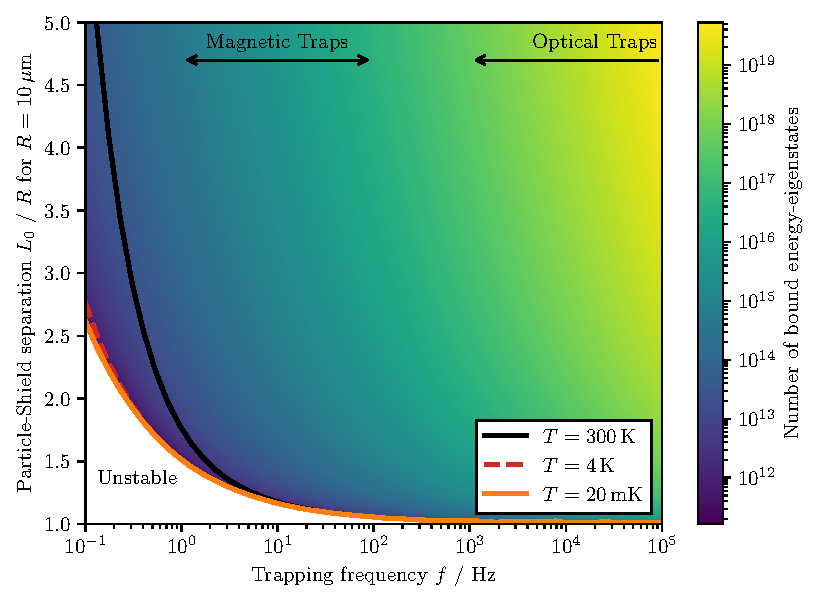
\includegraphics[width=\textwidth]{./../figures/others/trap-stability-with-R.pdf}
  \caption{Stability diagram for different trapping frequencies $f = \omega/2\pi$ and particle-shield separations $L_0$. The number of bound energy-eigenstates for each combination of $f$ and $L_0$ are calculated using the WKB-approximation. The number of thermally occupied states $\bar{n}$ at different Temperatures is overlaid. As an example, for $f=1\si{Hz}$, $\bar{n}(T=300\si{K})\approx 10^{13}$ states are thermally occupied. All regions below these boundaries are unstable. An increase in the radius $R$ and thus the mass $M$ improves the regions of stability massively.}
  \label{fig:4:trap-stability}
\end{figure}
In these calculations, tunneling effects through the potential boundary at $E_0$ are neglected, as they should not influence the results much considering the large number of bound eigenstates.
It turns out, that regardless the type of the trap, a successful trapping even at room temperature should be possible as long as the particle is placed appropriately far away from the trap.
The ability to trap and levitate the masses is therefore not significantly impaired by the presence of the Faraday shield.